\section{Compiling to Brainf*ck}
\subsection{Introduction to Acus}
A full computing environment is not complete without a compiler that generates the machine code from some human readable programming language. One could argue that Brainf*ck \emph{is} the programming language, but to say it's human readable is a bit of a stretch. The aim of this chapter is to describe the fundamentals behind the Acus library, which exposes a set of elementary assembly-like instructions (like arithmetic operations, conditional expressions and jumps) that are compiled into BF. Acus is meant to be used a compiler back-end: a layer that accepts higher-level operations and emits BF code. Since BF is lacking arbitrary code-jumps or memory accesses, familiar concepts like (possibly recursive) function-calls and pointer arithmetic are non-trivial. Multiple abstractions had to be built on top of the raw BF tape-cells in order for jumps and random memory access to be simulated at runtime.

\subsection{Program Structure}
In the Acus model, a program consists of a series of basic blocks, sequences of code that are always executed in order, and jumps between those blocks. Each basic block is compiled into its corresponding BF instructions and wrapped in a BF loop-pair (i.e.  between\texttt{[} and \texttt{]}) whose entry is controlled by generated guard code. The complete sequence of blocks is enclosed in a main-loop, conditional on the value in a special BF-cell, the \emph{Run}-cell, which can be reset by any block when the program should be terminated:

\begin{center}
  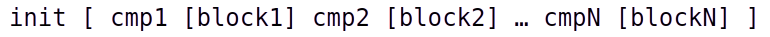
\includegraphics[width=0.8\textwidth]{img/program_structure}
\end{center}


The aforementioned guard-code compares the value of another predefined cell, the \emph{TargetBlock}-cell, to the block-index of the code-block. Only when this cell contains the exact index of the block \emph{and} the \emph{Run}-cell is still nonzero, is the loop entered and its code executed. Therefore, each block should at some point set the index of next block to be executed to keep the program going. This approach basically implements a state-machine that can be expressed in pseudo-code as shown in Listing \ref{lst:acusprogram}. Note that, on each iteration of the main-loop, all blocks are scanned until the scheduled block is encountered. In a worst-case scenario, when block \texttt{i} is scheduled by block \texttt{i+1} (the currently exectuted block), the system will first need to check all blocks from \texttt{i+2} up to \texttt{N} before looping back to block 1 and eventually block \texttt{i}.

\begin{lstfloat}[H]
  \begin{lstlisting}[style=pseudocode]
    blocks = [block1, block2, ..., blockN]

    Run = 1
    TargetBlock = 1 // not necessarily block 1

    while Run:
      for index = 1 ... N:
        if Run AND TargetBlock == index:
          execute blocks[index] 
  \end{lstlisting}
  \caption{Pseudocode of an Acus-generated program.}
  \label{lst:acusprogram}
\end{lstfloat}

\subsubsection*{Example: Fibonacci}
To illustrate how a program is divided into basic blocks, a simple fibonacci number generator is shown in Figure \ref{fig:fibexample}. It consists of three functions, each of which contains multiple basic blocks. The block-ID's are shown in square brackets at the start of each block. Blocks end at control-boundaries, i.e.~ places in the code where potential jumps take place or explicitly at predefined labels.

The program starts execution in block 10, which is set as the entry-point by the initialization code (note that initialization code of Listing \ref{lst:acusprogram} sets the entry-point to block 1; the specific example from below requires the initialization sequence to set this value to 10 instead). A function-call is immediately encountered, ending the current block. After initializing a new stack frame (this will be covered later, Section \ref{sec:noideayet}), the \emph{TargetBlock} is set to block 1: the entry-block index of the callee. This will cause control flow to skip over block 11 and loop back to block 1, which will then be entered. When control hits the conditional statement of block 3, either block 4 or 5 will be set as the next target-block, depending on the result of evaluating \texttt{i<n}. In this case, both the \texttt{if}- and \texttt{else} body contain only a single block that immediately terminates in a jump. When control eventually reaches the end of \texttt{main}, the \emph{Run}-cell is set to zero, causing flow to exit the main loop and terminate the program.

\begin{figure}[H]
  \centering
  \begin{subfigure}{0.4\linewidth}
    \centering
    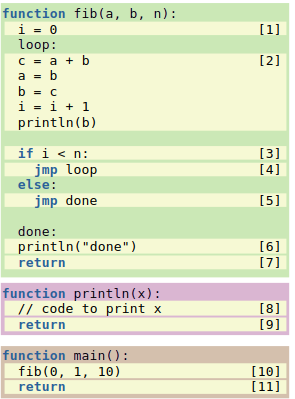
\includegraphics[height=10cm]{img/fib_blocks}
    \caption{Fibonacci program}
    \label{fig:fibblocks}
  \end{subfigure}
  \hspace{1cm}
  \begin{subfigure}{0.4\linewidth}
    \centering
    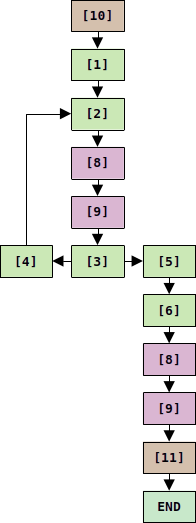
\includegraphics[height=10cm]{img/fib_flow}
    \caption{Control flow}
    \label{fig:fibflow}
  \end{subfigure}
  \caption{Figure (a) shows a simple fibonacci program (unspecified syntax) and how that program is split into blocks. Figure (b) shows how control flows from one block to another.}
  \label{fig:fibexample}
\end{figure}

\subsection{Tape Abstractions (Overview)}
The data-tape is considered a stack, where each function owns a stack frame. Each frame contains a return-slot (if the function returns a value), argument-slots (if the function takes arguments) and local data (variables and temporaries used in the function). A slot is a series of (logical) cells that contains a variable of some data-type, used by the function. The size of a slot depends on the number of cells required to represent the type of the variable. Instead of using single BF-cells to compose slots, logical cells or macro-cells are used. Each macro-cell contains 9 actual BF-cells, referred to as \emph{fields} from now on, each of which serves a different purpose. Central to the macro-cells are the two value-fields that hold the actual value of the logical cell. By having two value fields, we allow for 16-bit datatypes to be implemented within the same logical-cell, rather than having to allocate two macro-cells for a single 16-bit variable. The other fields hold temporary data or metadata required to perform higher level functions like arithmetic, flow control and dynamic pointer movement. When the compiler needs to generate code that moves the BF-pointer to location known only at runtime (for example when dereferencing pointers or accessing array elements by a dynamic index), these fields can hold temporary values or metadata necessary to perform the move. Other non-value fields include temporary scratch-pads (heavily used when performing arithmetic operations), payload-fields (used to transport data to locations known only at runtime) and a flag cell that is dedicated to the evaluation of loop-conditions. Having all these fields near one another on the BF-tape has the nice consequence of BF-algorithms being relatively short due to tight pointer-move-sequences.

\subsubsection*{Example: Fibonacci (continued)}
Figure \ref{fig:tapehierarchy} shows the tape hierarchy described above, applied to the fibonacci example from before and evaluated immediately after \texttt{fib} was first called. Even though this program made no use of any global data, this frame is still depicted for completeness' sake. Zooming in on Frame 2, used by the \texttt{fib}-function, we see how a frame starts with the slots we previously encountered in Section \ref{sec:compiling:program}: the \texttt{TargetBlock} and \texttt{Run} slots, which are used to determine where to jump next and whether to continue execution at all. Since \texttt{fib} does not return anything, no return-slot has been allocated to this frame. Instead, the local data immediately follows: first the arguments passed to the value (initialized by the caller), then the local data used within the function. Only the variables \texttt{c} and \texttt{i} have been explicitly allocated by the programmer, but temporary slots have been created by the compiler to store the result of \texttt{a + b} and \texttt{i < n}.

Zooming in further on two of the slots, we see that they both contain only a single macro-cell and its 9 constituents. The first slot of the frame (\texttt{TargetBlock}), which still holds ID 1 (the block-ID of the first block of the function) in its value-field, also has its \texttt{FrameMarker} field set, indicating that this is where a new frame starts on the data-tape. The \texttt{b}-slot has its value-field set to 1 as well, corresponding to the value of \texttt{b} that was passed to \texttt{fib} from \texttt{main}. 

Sections \ref{sec:compiling:first} through \ref{sec:compiling:last} below will go into more detail about each of the layers of abstraction.

\begin{figure}[H]
  \centering
  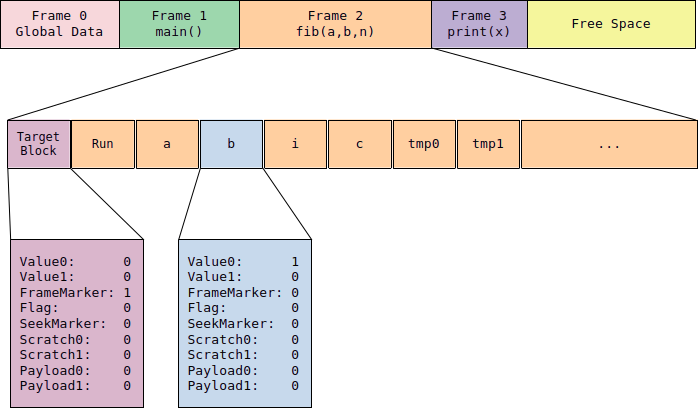
\includegraphics[width=0.8\textwidth]{img/tape_hierarchy}
  \caption{Acus tape hierarchy: the tape is divided into frames, which are divided into slots, which consist of macro-cells containing 9 fields (BF-cells).}
  \label{fig:tapehierarchy}
\end{figure}

\subsection{Cells and Macro-Cells}
BF operates on the most fundamental level of raw cells. Each consecutive sequence of 9 such cells constitutes a logical macro-cell as mentioned before in Section \ref{sec:compiling:tape}. In this section, we will cover each of the 9 fields of a macro-cell in more detail and cover some of their use cases. 

\subsubsection{\texttt{Value0} and \texttt{Value1}}
The value fields together hold the semantic value of the macro-cell. The \texttt{Value0} field contains the low byte and the the \texttt{Value1} field holds the high byte of an integer of at most 16 bits. Acus implements four integer data-types using these two fields: unsigned 8-bit (\texttt{u8}), unsigned 16-bit (\texttt{u16}), signed 8-bit (\texttt{s8}) and signed 16-bit (\texttt{s16}). When referring to 8-bit values, the \texttt{Value1} field is simply ignored. Signed integers are represented using two's complement; some algorithms need to do some additional work (like evaluating the sign-bit) before applying the usual operations.

\subsubsection{\texttt{Scratch0} and \texttt{Scratch1}}
Many BF algorithms need temporary cells as scratch-pads. These cells can be temporarily claimed by an algorithm and must be left behind empty for the next algorithm to use. An example of a simple algorithm that makes use of these values is the non-destructive addition. Say we want to add the contents of cell \texttt{x} to those of cell \texttt{y} without destroying \texttt{x} in the process. We can achieve this by decrementing \texttt{x} while at the same time incrementing \texttt{y} until \texttt{x} becomes zero. However, in order to restore \texttt{x} to its original value, we need to use a scratch-pad to construct a copy of \texttt{x} which is moved back after the addition has been completed. This algorithm is shown in Listing \ref{lst:bfadd}, where instead of denoting pointer-movement with sequences of \texttt{<} and \texttt{>}, we simply write the name of the variable/slot to indicate a move to that (known) location on the tape.

\begin{lstfloat}[H]
\begin{lstlisting}[style=brainfuck]
  # Algorithm for y += x
  # tmp is a scratch-cell assumed 0

  # Step 1: add x to both y and tmp, destroying x
  x[- y+ tmp+ x]

  # Step 2: add tmp back to the now empty x
  tmp[- x+ tmp]
\end{lstlisting}
\caption{Non-destructive addition of one cell to another, using a temporary scratch cell.}
\label{lst:bfadd}
\end{lstfloat}

\subsubsection{\texttt{Flag}}
The \texttt{Flag} field is reserved to store a value that determines whether or not a BF-loop should be entered. An algorithm can store an intermediate, temporary, value in the flag-cell and use that as a branch or loop-condition. Whereas scratch-cells are general purpose temporary storage locations, the flag-cell is meant to be used for this purpose alone to avoid confusion. The section below includes an example that also utilizes this field in Listing \ref{lst:bfseekframe}.

\subsubsection{\texttt{FrameMarker}}
The \texttt{FrameMarker} field is only set when the macrocell marks the start of a new frame. When performing dynamic pointer movements, a marker like this (the \texttt{SeekMarker} is used in a similar way) can be used to move from a still unknown to a known location on the tape. Let's say we know the data-pointer is somewhere in Frame 2, but we don't know where because we just performed some (dynamic) movement (i.e. an algorithm that moves the pointer by an amount that depends on runtime data). We know that the start of the frame is to the left of the current position, so we can perform the algorithm below and be sure that we're pointing at the start of the frame when the algorithm is finished. This algorithm is shown in the pseudo-BF of Listing \ref{lst:bfseekframe}. This works because every macro-cell has the same width and because exactly one FrameMarker is set at the start of the active frame.

\begin{enumerate}
\item Move the pointer to the \texttt{FrameMarker} field of the current cell. Even though the current offset is unknown, the current field \emph{is} known so we are able to switch between fields reliably.
\item Construct the logical \texttt{NOT} of the \texttt{FrameMarker} and store the result in the \texttt{Flag} field, then move the pointer to the \texttt{Flag} field.
\item Enter a loop, conditioned on the flag, where the pointer is moved 9 cells to the left on each iteration until a non-zero \texttt{FrameMarker} is encountered. In each iteration, the logical \texttt{NOT} has to be constructed and stored in the \texttt{Flag} field as before. Note that when inside a loop (meaning the flag was nonzero), the flag needs to be cleared before moving to the adjacent cell.
\end{enumerate}


\begin{lstfloat}[H]
  \begin{lstlisting}[style=brainfuck]
    # Algorithm to move the pointer back to the start of the frame
    # Current macro-cell offset is unknown; all moves are relative
    # field-switches within the same macro-cell, except for the
    # 9 left-moves, which take us exactly one macro-cell to the left.

    # Assumed: there already exist implementations for assignment and
    #          the logical NOT operator.
    
    ASSIGN(Flag, NOT(FrameMarker))
    Flag [-                            # Reset flag before moving away from it
      FrameMarker  <<<<<<<<<           # Move to the frame-marker field of neighboring macro-cell
      ASSIGN(Flag, NOT(FrameMarker))   # Compute exit-condition
      Flag                             # Check exit-condition
    ]

    # Out of the loop: pointer is at the start of the frame
  \end{lstlisting}
  \caption{Algorithm to seek left to the start of the current frame from an unknown initial position.}
  \label{lst:bfseekframe}
\end{lstfloat}

\subsubsection{\texttt{SeekMarker}}
The purpose of the \texttt{SeekMarker} field is very similar to that of the \texttt{FrameMarker} field, in the sense that it is used to mark certain cells to make dynamic movement possible. For example, a known location can be marked before performing a dynamic move, in order to be able to move back to that known location using an algorithm similar to that of Listing \ref{lst:bfseekframe}. Also, when a dynamic move has been completed, its location can be marked to make future excursions to this location more efficient. Contrary to the \texttt{FrameMarker}, which is specifically used to mark the start of a frame, the \texttt{SeekMarker} field may be set for any macro-cell on the tape.

\subsubsection{\texttt{Payload0} and \texttt{Payload1}}
The payload fields are used to store values that need to be transported along to dynamically determined locations. Algorithms that move the pointer to such locations can be trivially extended to move data along using these fields: one for the low byte and one for the high byte of the value. Additionally (but this is not the intended use-case), a payload cell may be used as a scratch-pad (when an algorithm has exhausted the available scratch cells), provided it is not being used to transport any values at that time.

\subsection{Slots}
A slot is a storage location for one value. Single 8 or 16-bit integers occupy a single macro-cell, while larger values like arrays or structs occupy a sequence of macro-cells. A slot is bound to a stack frame; its offset is defined as the index of its first macro-cell with respect to the start of the frame, not the start of the actual BF data-tape.

In addition to a name and offset, a slot holds information about its scope (to determine access, allow for name-shadowing and keep track of lifetime) and its \emph{kind}. Most slots are of the \emph{local} kind, representing data local to the current function, but slots can also be tagged \emph{global}, \emph{available} (representing a free block of memory that was previously occupied), \emph{temp} (for temporary slots that should be freed after use) and \emph{cache} (Section \ref{sec:compiling:cache}). Figure \ref{fig:slots} shows a section of a frame and how local slots could be organized given their data-types and sizes. Note that the size of a slot is expressed in terms of the number of macro-cells rather than raw BF cells.

\begin{figure}[H]
  \centering
  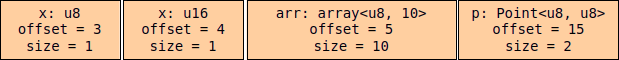
\includegraphics[width=0.8\textwidth]{img/slots}
  \caption{Slots represent variables, which may span multiple macro-cells.}
  \label{fig:slots}
\end{figure}

\subsubsection{Slot Proxies and Materialization}
Most expressions encountered by the compiler can be resolved directly into a slot. For example, assume \texttt{x} is an array of structs that contain an \texttt{age} field, e.g. 

\begin{lstlisting}
  struct Person {
    id:  u16
    age: u8
  };

  let x: array<Person, 5>;
\end{lstlisting}

In this context, the expressions \texttt{x}, \texttt{x[2]} and \texttt{x[2].age} all refer to known slots or sub-slots (assuming square brackets represent array indexing and a dot represents field access for struct objects). The compiler knows in which slot the array \texttt{x} is stored, it knows how to find the offset of element 2 and it knows how to find the offset of the \texttt{age} field.

However, when the index is not a compile-time constant, things change. The expression \texttt{x[i].age} has the same shape as \texttt{x[2].age} (they might even refer to the same data), but now the compiler has no way to compute the desired offset at compile-time. At this point, the expression can no longer be represented by a single statically known slot. The array itself still has a known base location, and the layout of each \texttt{Person} object is still known, but the particular element that should be accessed depends on a value computed at runtime. In Brainfuck terms, the compiler must now generate code that moves through the tape dynamically, using the value of \texttt{i} to reach the correct element before applying the fixed offset of the \texttt{age} field.

This is where Acus introduces the notion of a \emph{slot proxy}. A slot proxy is not necessarily a slot by itself, but a description of how a value can be accessed. Some proxies are direct: they simply refer to an already known slot. Others are indirect: they describe an access path that must be resolved at runtime. The expression \texttt{x[2].age} can be reduced to a direct sub-slot, while \texttt{x[i].age} becomes a proxy that says, in effect: start from the slot occupied by \texttt{x}, use the runtime value of \texttt{i} to select an element, and then access the \texttt{age} field within that element. In general, modifications made to that element (e.g. \texttt{x[i].age += n}) will need a read-modify-write cycle where the element is first \emph{materialized} into a known, temporary slot (much like a hardware register), modified and written back using a dynamic write-algorithm. This process of materialization and write-back is shown conceptually in Figure \ref{fig:materialization}.

\begin{figure}[H]
  \centering
  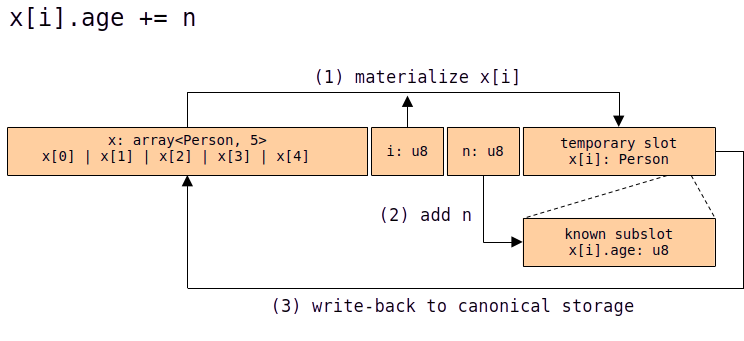
\includegraphics[width=0.8\textwidth]{img/materialization}
  \caption{Materialization process for a modification to a dynamically indexed array.}
  \label{fig:materialization}
\end{figure}


The distinction between actual slots and proxies that represent them allows the compiler to treat simple variables, struct fields, array elements and pointer dereferences in a uniform way. Code that needs to read from or write to an expression does not have to know immediately whether the target is a fixed slot or a dynamically computed location. It can ask the proxy to materialize the value into a concrete slot, or to write a concrete value back through the described access path.

For the purposes of this chapter, slot proxies should therefore be understood as compiler-level access paths. They bridge the gap between the static memory layout known at compile-time and the dynamic addresses that sometimes have to be computed at runtime. This idea becomes especially important in the caching system (Section \ref{sec:compiling:cache}), which is designed to limit unnecessary materialization and synchronization events.

\subsubsection{Local Memory Management}
Section about local stack data and the memory management system that keeps the stack frames tightly organized.

\subsection{Stack Frames and Function Calls}
A frame groups all data belonging to one function activation. Each frame contains the local control cells, optional return storage, arguments, named locals and compiler-generated temporaries (and cached values). Function calls can then be viewed as transitions between frames: the caller prepares the callee frame, moves the data-pointer to the start of the frame and sets the \texttt{TargetBlock} value to the callee's entry block. When a function returns, the data-pointer is moved back to the caller's frame and execution continues at the first block beyond the call. Each of these steps will be described in more detail in the sections below.

\subsubsection{Reference Frames}
Each stack frame acts as a frame of reference, or coordinate system, to the data-pointer. Since function calls happen dynamically, stack frames are allocated dynamically as well. This means that the compiler has no way of knowing where the data-pointer is located in an absolute sense (i.e. with respect to the start of the BF-tape). Instead, it keeps track of the pointer-location with respect to the start of the current frame. Pushing a new frame on top of the stack and moving the pointer to the start of this frame can then be seen as performing a coordinate transformation - or rebase - of the pointer: the origin is now in the frame of the callee rather than the caller. 

\subsubsection{Global Data Frame}
Global data is allocated in its own frame at the very start of the data-tape, i.e. frame 0. This frame is not owned by any function and is accessible from any other frame to fetch data from or write to. Like dynamic array accesses or pointer dereferences, a global slot is accessed through a slot-proxy and will be materialized locally before any work can be done on it. This introduces synchronization issues accross call-boundaries, which will be addressed in Section \ref{sec:compiling:cache}. In the sections below, the concept of (stack) frames refers to a frames actually tied to the functions being executed, not the global frame.

\subsubsection{Frame Layout}
The exact layout of a frame depends on the nature of the function that it belongs to, depending on the return-type and number of arguments it takes. However, each instance of a function-call will cause an identical frame-layout to be generated as a result. In general, a frame is laid out as follows (in terms of macro-cells):
\begin{enumerate}
\item \texttt{TargetBlock}: a macro-cell who's \texttt{Value} fields are set to the index of the next block scheduled for execution and who's \texttt{FrameMarker} is set to 1, indicating the start of a new frame.
\item \texttt{Run}: a macro-cell dedicated to store a local copy of the program's \emph{run}-state. As soon as this flag is set to 0 (from any frame), none of the blocks will execute and the main loop will be aborted.
\item \texttt{ReturnSlot}: Depending on the return-type of the function, a slot is allocated to hold the return-value. Note that this slot is located at a fixed offset, so it can be reached easily even from within the caller's frame in order to fetch the return-value. If the function returns \texttt{void}, this slot does not exist at all.
\item \texttt{Locals}: Data local to the frame, which can be categorized further:
  \begin{enumerate}
  \item local variables (including function-arguments), organised in slots as discussed before in Section \ref{sec:compiling:slots}.
  \item compiler-generated temporaries
  \item cached materializations
  \end{enumerate}
\end{enumerate}

\subsubsection{Calls and Returns (meta-blocks)}
\paragraph{Calls} To call a function, the caller has to perform the following actions:
\begin{enumerate}
\item Set the caller's \texttt{TargetBlock} to the ID of a compiler-generated meta-block. This is the continuation that will run after the callee returns (see Section \ref{sec:compiling:metablocks} below).
\item Copy or materialize the function arguments into the argument slots of the next frame. The offsets are known relative to the caller's frame, so this does not require a runtime search.
\item Initialize the control cells of the callee frame: its \texttt{Run} cell is set and its \texttt{TargetBlock} is set to the callee's entry block.
\item Move the data pointer to the start of the callee frame and treat this position as the new origin.
\end{enumerate}
After these steps, the runtime naturally dispactches to the block who's ID is now stored in the \texttt{TargetBlock} cell of the freshly initialized stack frame.

\paragraph{Meta-blocks} These are compiler-generated code-blocks that are scheduled at the time of the call, while still in the caller's frame. When the pointer is popped back to this frame after the callee returns, this is the value that is observed and used to determine the next block to be executed. This block is then responsible for making sure that
\begin{enumerate}
\item the return value is fetched from the callee's frame and copied into the return-slot of the caller (if provided; it may also be ignored),
\item the state of the \emph{run}-flag is copied back into the caller's frame (to propagate its state in case the callee changed it), and 
\item the \texttt{TargetBlock} cell is set to the ID of the block following the call.
\end{enumerate}

Propagatin the \emph{run}-flag like this makes early termination compositional: if a callee stops the program, the caller observes the same stopped state after the return metablock has run. This allows a (builtin) function like \texttt{abort()} to be implemented.

\paragraph{Returns} To return control to the caller, we only need to make sure that the return-slot is populated appropriately and pop the data-pointer back to the frame below. The meta-block has already been scheduled and will take control immediately, finishing the transaction as described above.

Figure \ref{fig:call_return} shows data transfers and the setup that occurs while performing a call and returning from it. At the call-site, the target-blocks are set and arguments are copied over to the next frame. When returning and control has been passed to the meta-block, return-data is copied back from the callee's frame into the current one.

\begin{figure}[H]
  \centering
  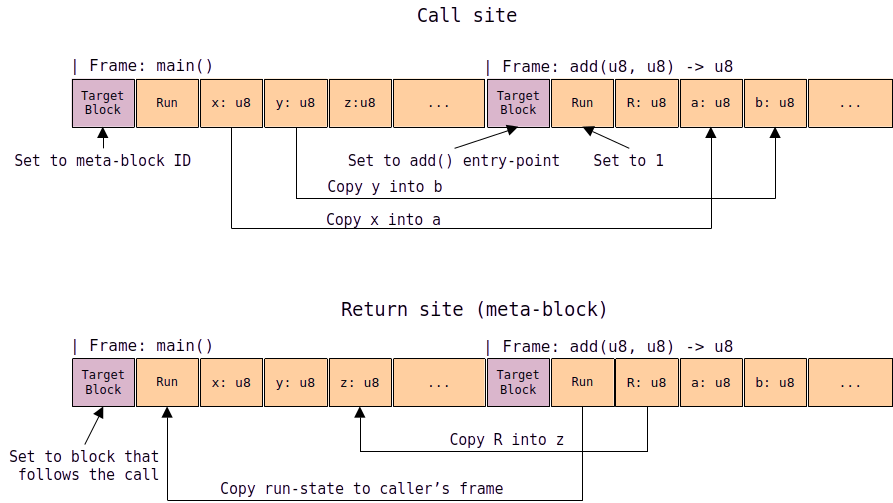
\includegraphics[width=0.8\textwidth]{img/function_call_return}
  \caption{Conceptual overview of data-tape manipulations that occur when calling a function and returning from it. This graphic assumes that in between these two moments, the \texttt{add} function has populated the return-slot (\texttt{R}).}
  \label{fig:call_return}
\end{figure}

Notice that the return address is not stored on a hardware stack. It is encoded as a block ID in the caller’s \texttt{TargetBlock} cell. Returning to the caller therefore means restoring the caller frame; the scheduler will then execute the metablock whose ID was already waiting there.




\subsection{Code Generation Patterns}
This section should introduce the small set of BF idioms from which larger operations are assembled. It should not become a catalogue of every algorithm in the compiler. Instead, it should show enough examples to make the generated code feel less magical.

\subsubsection{Clearing, Moving and Copying Values}
The simplest useful BF idiom is destructive movement: consume one cell while adding its value somewhere else. From that, one can build clearing, moving and non-destructive copying by introducing temporary storage. These operations are worth including because they appear everywhere: assignments, argument passing, return values and arithmetic all rely on them.

\paragraph{Suggested figure.}
Use a before/after tape diagram showing a destructive move from cell \(A\) to cell \(B\), followed by a non-destructive copy using a temporary cell. This can be shown without writing the full BF sequence.

\subsubsection{Addition and Subtraction}
Addition and subtraction are the natural next step after copying. For small values, they are implemented by transferring counts between cells; for multi-cell values, the algorithm has to propagate borrow or carry between macro-cells. This subsection should explain why arithmetic on a BF tape is not a single operation but a choreography of local loops.

Include addition and subtraction as the main arithmetic examples. They are fundamental enough to justify space, while multiplication and division can be mentioned only briefly as repeated or derived algorithms unless they become important in a later case study.

\paragraph{Suggested figure.}
A two-row diagram works well here: the first row shows single-cell addition, the second row shows multi-cell addition with a carry flag moving to the next macro-cell.

\subsubsection{Comparison and Boolean Results}
Conditionals and loops require values to be converted into flags. The most useful comparisons to feature are zero/nonzero, equality and less-than. These are enough to explain how high-level control flow becomes BF block selection: the comparison produces a boolean value, and that value is then used to choose the next target block.

This subsection should emphasize the output of comparison algorithms rather than every internal step. The reader should come away understanding that comparisons are compiled into ordinary tape transformations whose result is stored in a normal slot or flag cell.

\paragraph{Suggested figure.}
Show an expression such as \texttt{i < n} being lowered into a temporary boolean slot, followed by a block-selection decision. This connects the arithmetic section back to the program-structure section.

\subsubsection{Selected Algorithms to Omit or Defer}
Do not spend chapter space on every operation Acus can generate. Multiplication, division, modulo, string formatting and input parsing can be summarized in a short paragraph or deferred to examples if needed. The chapter will be stronger if it focuses on the operations that reveal the underlying model: move/copy, add/subtract, compare and dynamic pointer movement.

\subsection{Pointer Movement}
BF has no random access instruction; the only way to reach a cell is to move the pointer step by step. This makes pointer movement one of the central code-generation problems in Acus. The compiler must constantly choose between generating a known relative move and generating a runtime search or traversal.

\subsubsection{Static Pointer Movement}
When the source and destination locations are known at compile time, pointer movement is straightforward: emit the required number of \texttt{<} or \texttt{>} commands. This is the common case for local slot operations within a frame. The compiler can keep track of the current pointer position and avoid unnecessary moves by scheduling nearby operations together where possible.

\paragraph{Suggested figure.}
Show a tape with a current pointer position and a target slot at a known offset. Annotate the resulting BF movement as a fixed sequence of arrows.

\subsubsection{Frame-Relative Movement}
Most ordinary local variables can be addressed relative to the current frame. This subsection should explain the role of frame markers and known frame layouts: even though the underlying BF tape is flat, Acus imposes structure on it so that generated code can move predictably within the active frame.

This is a good place to connect the frame abstraction to the cost of generated code. A variable that is close to the current pointer is cheap to access; one that is far away requires a longer sequence of moves. The layout of frames and temporaries therefore directly influences the generated BF size.

\paragraph{Suggested figure.}
Show the same function frame twice: once as an abstract frame with named slots, and once as a linear tape with offsets from the frame marker.

\subsubsection{Dynamic Pointer Movement}
The most interesting pointer-movement algorithms are the ones where the target is not known until runtime. Examples include array access by a computed index, pointer dereferencing and moving data to a slot selected by a runtime value. These algorithms rely on metadata stored in macro-cells: markers, counters and payload fields are used so that the BF pointer can search through structured tape data and stop at the correct logical cell.

This is the pointer-movement algorithm most worth featuring in detail. It captures the central difficulty of compiling to BF: the target address is not available as an address, so it must be represented as data on the tape and consumed by a traversal algorithm.

\paragraph{Suggested figure.}
Show an array slot with several elements and an index value stored elsewhere. Then show a runtime traversal in which the index is decremented while the pointer advances from element to element until the selected element is reached.

\subsubsection{Payload Transport}
Dynamic writes are harder than dynamic reads because data has to be carried to a location that is not statically known. Acus solves this by moving values through designated payload fields. The payload travels along with the dynamic traversal and is deposited when the target macro-cell is found.

This subsection should describe the idea at a high level, because it is one of the more distinctive algorithms in the compiler. It also gives a natural explanation for why macro-cells contain more than just value storage.

\paragraph{Suggested figure.}
Use a three-stage diagram: prepare payload, traverse to dynamic target, commit payload into the selected value field.

\subsection{Control Flow and Functions}
This section should tie the earlier pieces together: arithmetic produces flags, flags select blocks, blocks update the target-block cell, and function calls are represented as jumps between frames.

\subsubsection{Conditionals}
An \texttt{if}-statement becomes a small control-flow graph. First, the condition expression is evaluated into a temporary boolean slot. Then the current block selects one of two successor blocks. Both branches eventually continue at a join block, unless they return or jump elsewhere.

\paragraph{Suggested figure.}
A minimal control-flow graph for \texttt{if/else}: condition block, then block, else block and join block. This should visually resemble Figure~\ref{fig:fibflow}.

\subsubsection{Loops}
A high-level loop is compiled as a cycle in the block graph. The condition block either jumps into the body or exits to the block after the loop. The body eventually jumps back to the condition block. \texttt{break} and \texttt{continue} are then just additional edges in this graph.

\paragraph{Suggested figure.}
Show a loop as four blocks: preheader, condition, body and exit. Add dashed arrows for \texttt{break} and \texttt{continue}.

\subsubsection{Function Calls and Returns}
A function call consists of preparing the callee frame, copying arguments into it, storing enough return information to resume the caller, and selecting the callee's entry block. Returning reverses this process: the return value is written to the caller's expected location, the caller frame becomes active again, and the target block is set to the continuation block.

Keep this subsection conceptual. The aim is to explain that calls and returns are not BF primitives but conventions implemented on the tape and in the block scheduler.

\paragraph{Suggested figure.}
A timeline figure would be useful: caller before call, callee active, caller after return. Indicate how the active frame changes and where the return value goes.

\subsection{Caching and Materialization}
\label{sec:compiling:cache}
The caching system is the one implementation-oriented topic worth treating in more depth, because it explains how Acus avoids generating an excessive amount of BF for repeated accesses to the same logical values. Without caching, every read and write would immediately synchronize all relevant tape locations, leading to large and slow programs.

\subsubsection{The Problem: Repeated Materialization}
Slot proxies allow expressions to remain abstract until their value is needed. However, repeatedly materializing the same proxy can duplicate work. For example, accessing the same array element or struct field several times in a block should not require recomputing the entire access path each time.

This subsection should present the problem using a simple expression such as \texttt{x = a[i] + a[i]}. The compiler should recognize that both occurrences refer to the same logical location, while still being conservative when aliases or writes might invalidate that assumption.

\paragraph{Suggested figure.}
Show two identical proxy trees leading to the same materialized slot. Then show the optimized version where the first materialization is reused.

\subsubsection{Cache Entries}
A cache entry connects a logical proxy to a concrete slot that currently holds its materialized value. The cache is therefore not merely a value cache; it is a bridge between abstract access paths and physical tape storage. Entries can be clean, dirty or invalid depending on whether the concrete slot agrees with the underlying logical location.

This subsection may include a little more detail than the rest of the chapter, but it should still be written in terms of invariants rather than C++ classes. The key invariant is that generated BF must observe the same values as if every proxy access were performed directly.

\paragraph{Suggested figure.}
Use a table-like figure with columns \emph{proxy}, \emph{materialized slot}, \emph{state} and \emph{meaning}. Keep it small: three or four entries are enough.

\subsubsection{Reads, Writes and Dirty State}
Reads may reuse a clean cache entry. Writes are more subtle: writing through one proxy may invalidate cached values for the same location or for locations below it in the proxy tree. A write can also make a materialized slot dirty, meaning that its value must eventually be committed back to the underlying location.

This is the place to explain parent/child invalidation at a conceptual level. For example, writing to an array element should invalidate cached views of that element and possibly cached views of the containing array, depending on what assumptions the cache had made.

\paragraph{Suggested figure.}
Show a proxy tree for an aggregate value. Highlight the subtree invalidated by writing to one child element.

\subsubsection{Boundaries}
The cache is allowed to be clever only where control flow and aliasing are under control. At function calls, jumps and other control boundaries, Acus conservatively flushes or invalidates cached state. This mirrors the role of synchronization in the Synapse-191 hardware: values may temporarily live in a faster or more convenient representation, but they must be made consistent before the next part of the program relies on them.

A useful comparison can be made here to the A and V flags from the hardware chapter. Synapse-191 tracks whether the data-pointer or data value has changed so it can avoid unnecessary RAM traffic; Acus generalizes this idea from one hardware register to many compiler-managed tape locations.

\paragraph{Suggested figure.}
Show a block with several cached operations internally, followed by a control boundary where dirty entries are flushed and uncertain entries are invalidated.

\subsubsection{Aliasing and Conservative Choices}
The hardest cache cases arise when two different proxies might refer to the same storage, such as through pointers or dynamic array indices. Acus should prefer correctness over cleverness here. When a write may be visible through another access path, the cache must assume that related entries are no longer trustworthy.

This subsection should be honest about the trade-off: conservative invalidation can generate more BF, but it prevents subtle wrong-code bugs. This is also a good place to mention that pointer writes are deliberately treated as immediate visibility boundaries.

\paragraph{Suggested figure.}
Show two different access paths converging on the same slot: one through a named variable, one through a pointer. Mark the cache entries that become invalid after the pointer write.

\subsection{Selected Case Studies}
Rather than listing every supported language feature, this section should use a few examples to show how the previous ideas combine. Each case study should be short and should include either generated BF statistics, a tape diagram, or a control-flow diagram.

\subsubsection{A Small Arithmetic Example}
Use a compact program that computes a value using assignment, addition, subtraction and comparison. The goal is to connect slots, temporaries, arithmetic idioms and block selection in one example.

\paragraph{Suggested figure.}
A side-by-side view: high-level pseudocode on the left, simplified block graph or tape effects on the right.

\subsubsection{Dynamic Array Access}
This is the best pointer-movement case study. An expression like \texttt{arr[i] = arr[i] + 1} involves dynamic reads, arithmetic and a dynamic write. It also stresses caching: the two appearances of \texttt{arr[i]} may be related, but the write must still be handled carefully.

\paragraph{Suggested figure.}
A sequence diagram showing materialize \texttt{arr[i]}, increment temporary, write back through dynamic traversal.

\subsubsection{Recursive Fibonacci}
The Fibonacci example already introduced block scheduling and frames, so it can be revisited here as a larger integration test. It demonstrates calls, returns, temporaries, conditionals and repeated frame creation. The section should focus on what the generated BF has to simulate, not on the C++ interface used to describe the program.

\paragraph{Suggested figure.}
Show a shallow recursion tree next to a stack frame diagram. This makes the cost of recursion on a BF tape concrete.

\subsection{Limitations and Trade-Offs}
This chapter should end by making clear that Acus does not make BF efficient in an absolute sense. It makes BF compilation systematic. The generated programs are large because every high-level operation must eventually become pointer moves, cell updates and loops. The value of the compiler is that it makes these transformations reliable and composable.

\subsubsection{Code Size Versus Runtime Work}
Some transformations reduce runtime work but increase program size, while others keep the generated BF short at the cost of more movement at runtime. Caching, temporary reuse and block layout all live in this trade-off space.

\subsubsection{Abstraction Versus Control}
The abstractions used by Acus make it possible to generate BF from structured programs, but each abstraction hides a cost. Frames, slots, proxies and caches are useful precisely because they make those costs manageable rather than invisible.

\subsubsection{Future Directions}
Close with a brief list of possible improvements: better block ordering, more precise alias analysis, more aggressive cache retention across safe boundaries, improved temporary allocation and more specialized arithmetic kernels. This should read as a natural continuation of the techniques in the chapter, not as a new implementation roadmap.

